\scanpage{38}
\deleted{\unsure{A}} Moyennant l'isom $(\unsure{\alpha})$, l'opération $L_Y$ s'identifie à $L_X$ sur le morceau
\[
\coprod_{\substack{i+j\leq n-2\\i,j\geq0}}L_X^jP^i(X),
\]
et son noyau est le morceau
\[
\coprod_{\substack{\deleted{\unsure{i+j}}\\i+j=n-1\\i,j\geq0}}\uline{L_X^jP^i(X)}\oplus E^{(n-1)}
=\coprod_{i\geq n+1}P^{\unsure{j|i}}(X)\oplus E^{n-1}
\]
(qui n'est d'ailleurs autre que $\displaystyle\coprod_{\substack{\deleted{\unsure{i\geq n}}\\n\leq i\leq2(n-1)}}P^i(Y)$, comme il se doit). L'opération $\Lambda_Y$ est nulle sur $E^{n-1}$, et coïncide sur le morceau
\[\coprod_{\substack{i+j\leq n-1\\i,j\geq0}}L_X^jP^i(X)\]
avec $\Lambda_X$. On retrouve \deleted{\unsure{l'injectivité|l'égalité}}\inserted{que le noyau} de $\Lambda_Y$ \deleted{\unsure{sur}} est
\[
\coprod_{\unsure{0\leq i\leq n-1}}P^i(X)+E^{n-1}=\coprod_{0\leq i\leq\unsure{n+1|n-1}}P^i(Y),
\]
\deleted{\unsure{donc}} et que $\Lambda_Y$ est injectif sur le reste
\[
=\coprod_{\substack{i+j\leq n-2\\\deleted{i\geq0,j>0}\\i,j\geq0}}L_X^{1+j}P^i(X).
\]
On en déduit
\deleted{
\[
\left\{\begin{aligned}
\deleted{\unsure{\Lambda_Y\varphi^*=\Lambda_X}}\varphi^*\Lambda_X&=\Lambda_Y\varphi^*+\\
\varphi_*\Lambda_Y&=\Lambda_X\varphi_*
\end{aligned}\right.
\]
Pour la \deleted{dernière}\inserted{\unsure{prem.}} relation, on la vérifie d'abord sur les $P^j(X)$ \inserted{$=$} pour $j\geq n$, \inserted{i.e. les $L_X^{n-i}P^i(X)$ pour $i\leq n-1$)} \deleted{le premier est} \unsure{y est nul} car $\varphi^*$ l'est, le deuxième
}
\figure{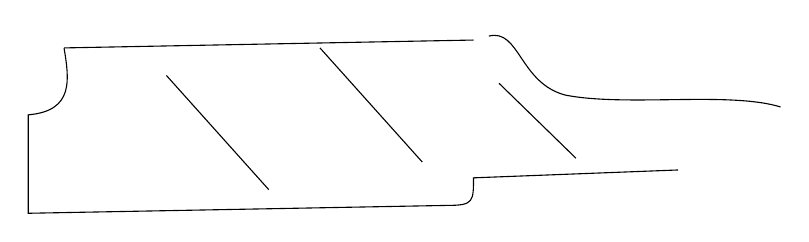
\begin{tikzpicture}[x=.65cm,y=.5cm]
\draw (0,0)--(8,.2);
\draw (0,0)..controls(.1,-.8)and(.2,-1.6)..(-.7,-1.7)--(-.7,-4.2)--(7.5,-4)..controls(8,-4)and(8,-3.9)..(8,-3.3)--(12,-3.1);
\draw (8.3,.3)..controls(8.9,.5)and(8.9,-.9)..(9.8,-1.2)..controls(11,-1.5)and(13,-1.1)..(14,-1.5);
\draw (2,-.7)--(4,-3.6);
\draw (5,0)--(7,-2.9);
\draw (8.5,-.9)--(10,-2.8);
\end{tikzpicture}}

\deleted{$\varphi^*\Lambda_X=$}
\[
\left\{\begin{aligned}
\Lambda_Y\varphi^*&=\varphi^*\Lambda_X\left(\operatorname{id}_X-\sum_{n+1\leq j\leq2n}p_X^j\right)
=\left(\operatorname{id}_Y\unsure{-}\sum_{\unsure{n-1|n+1}\leq j\leq2(n-1)}p_X^j\right)\varphi^*\Lambda_X\\
\varphi^*\Lambda_Xp_X^j&=p_Y^{j-2}\varphi^*\Lambda_X\deleted{\unsure{=p_Y^{j-2}\Lambda_Y\varphi^*}}
\qquad\text{si }j\geq n+1.
\end{aligned}\right.
\]
\margin{\[\Longleftarrow\quad\Lambda_Y^m\varphi^*=\varphi^*\Lambda_X^m(\operatorname{id}-\bar\Sigma)\]
pour tt $m$}
\[
\left\{\begin{aligned}
\varphi_*\Lambda_Y&=\left(\operatorname{id}_X-\sum_{0\leq i\leq n-1}p_X^i\right)\Lambda_X\varphi_*
=\Lambda_X\varphi_*\left(\operatorname{id}_Y-\sum_{0\leq i\leq n-1}p_Y^i\right)\\
p_X^i\Lambda_X\varphi^*&=\Lambda_X\varphi^*p_Y^i=p_X^i\varphi_*\Lambda_Y\qquad\text{si }0\leq i\leq n-1.
\end{aligned}\right.
\]
\mspage{37}
